\documentclass[11pt,letterpaper]{article}

% ---- packages ----
\usepackage[margin=1in]{geometry}
\usepackage{amsmath,amssymb,amsfonts}
\usepackage{booktabs}
\usepackage{graphicx}
\usepackage{hyperref}
\usepackage{url}
\usepackage{xcolor}
\usepackage[numbers]{natbib}
\usepackage{caption}
\captionsetup{font=small,labelfont=bf}

\hypersetup{colorlinks=true,linkcolor=black,citecolor=black,urlcolor=blue}

% ---- paths (adjust to your local clone) ----
\graphicspath{{../figures/}}
\newcommand{\RELAY}{\textsc{Relay}}

\title{\RELAY: Parallel Portfolio Racing for\\ Incomplete Weighted MaxSAT}
\author{Anonymous Author(s)}
\date{}

\begin{document}
\maketitle

\begin{abstract}
We introduce \RELAY\ (\underline{R}acing \underline{E}nsemble with \underline{L}earned \underline{A}lgorithm s\underline{Y}nthesis), a parallel-portfolio framework for the incomplete track of Weighted MaxSAT.  \RELAY\ executes $k$ off-the-shelf stochastic local-search (SLS) solvers concurrently on each instance and returns the minimum cost across solvers at the wall-clock deadline.  A single-core variant, \RELAY-RF, learns to predict the best solver per instance from twelve lightweight formula features.  Evaluated on MaxSAT Evaluation (MSE) 2020--2024 (1{,}736 matched instances), \RELAY\ \emph{strictly dominates} NuWLS --- the previously reported single-solver state of the art --- at both 60\,s and 300\,s timeouts, with hundreds of wins and \emph{zero} instance-level regressions.  A three-solver portfolio already exceeds NuWLS by $+2.00$ (absolute score, 60\,s, 241/0 W/L), closing 85\% of the gap to the eight-solver Virtual Best Solver (VBS) ceiling.
\end{abstract}

% ---------------------------------------------------------------
\section{Introduction}
% ---------------------------------------------------------------

Incomplete Weighted MaxSAT solvers aim to return the best-cost assignment they can find before a wall-clock budget expires.  The MaxSAT Evaluation (MSE) benchmark \citep{mse2020,mse2024} remains the standard testbed, and in recent years stochastic local search (SLS) solvers such as NuWLS \citep{nuwls2023} and SatLike~\citep{satlike} have dominated this track.  Neural-network methods that claim improvements over these SLS baselines typically report overall average scores that rely on a \emph{single} solver on the comparison side.

Single-solver comparisons, however, mask a simple structural observation: no single solver is uniformly best.  Different solvers excel on different instance families, and the \emph{Virtual Best Solver} (VBS) --- the per-instance oracle over a pool of solvers --- is noticeably stronger than the strongest individual member.  On modern multi-core hardware, the gap between a single solver and VBS can be recovered \emph{without} any neural modelling simply by racing a small handful of solvers in parallel.

We investigate this observation quantitatively.  Our contributions are:

\begin{enumerate}
    \item We introduce \RELAY, a parallel portfolio for incomplete MaxSAT that takes the per-instance minimum cost across $k$ concurrent SLS solvers.  \RELAY\ is a strict Pareto improvement over any individual member of the pool.
    \item We evaluate $k\in\{2,3,4,8\}$ on MSE 2020--2024 (1{,}736 matched instances) at both 60\,s and 300\,s budgets, and show \RELAY\ surpasses NuWLS by $+1.3\%$ to $+2.4\%$ absolute score with zero instance-level regressions.
    \item We propose \RELAY-RF, a single-core variant that uses a random-forest selector over twelve instance features to predict the best solver per instance with a confidence-gated fallback.
\end{enumerate}

% ---------------------------------------------------------------
\section{Background}
% ---------------------------------------------------------------

\paragraph{Weighted MaxSAT.}  A weighted MaxSAT instance is a finite multiset of weighted clauses $\{(C_j,w_j)\}$ in conjunctive normal form.  A clause is \emph{hard} if its weight exceeds a threshold $w_{\max}$ and \emph{soft} otherwise.  A feasible assignment satisfies all hard clauses; among feasible assignments, the goal is to minimise $\sum_{j\in U(\sigma)} w_j$, where $U(\sigma)$ is the set of unsatisfied soft clauses under assignment $\sigma$.

\paragraph{Incomplete-track scoring.}  MSE's incomplete track rewards approximate solutions: for each instance $i$, a solver reporting cost $c_i$ receives score
\[
    s_i \;=\; \min\!\left(1,\; \frac{1+c_i^{\star}}{1+c_i}\right),
\]
where $c_i^{\star}$ is the official MSE best-known cost.  The aggregate per (year, category) score is the instance mean.  We adopt this metric throughout.

\paragraph{Portfolios and VBS.}  Given a pool of $k$ solvers $\{S_1,\ldots,S_k\}$, the Virtual Best Solver assigns to instance $i$ the cost $c_i^{\text{VBS}} = \min_j c_i^{(j)}$.  VBS is not realizable without an oracle; the realistic realization is the \emph{parallel portfolio} that runs all $k$ solvers concurrently under a shared wall-clock budget.

% ---------------------------------------------------------------
\section{\RELAY: Parallel Portfolio Racing}
% ---------------------------------------------------------------

\subsection{Parallel portfolio (\RELAY-PP$k$)}

Given a pool $\mathcal{P}$ of $k$ SLS solvers with per-solver single-thread time budget $T$:

\begin{enumerate}
    \item Launch all $k$ solvers on the instance in parallel, each with budget $T$.
    \item Each solver is an anytime procedure: it prints monotonically improving incumbents $c_j(t)$ as $t$ grows.
    \item At deadline $T$, \RELAY\ returns $\hat{c} = \min_j c_j(T)$, i.e.\ the minimum incumbent across solvers at the wall-clock deadline.
\end{enumerate}

Because each $c_j(T)$ is bounded above by the solver's own individual cost, $\hat{c} \le c_j(T)$ for every $j$.  Consequently $\text{score}_{\text{\RELAY}} \ge \text{score}_j$ instance-by-instance, making \RELAY\ a strict Pareto improvement over every member of the pool.  Computational cost is $k$ CPU cores but wall-clock remains $T$.

\subsection{Pool construction}

We experiment with pools $\mathcal{P}_2 = \{\text{NuWLS}, \text{SPB}\}$, $\mathcal{P}_3 = \mathcal{P}_2 \cup \{\text{SatLike}\}$, $\mathcal{P}_4 = \{\text{NuWLS}, \text{NuWLS-c}, \text{SPB}, \text{SPB-c}\}$, and $\mathcal{P}_8$ comprising all eight evaluated solvers (see Section~\ref{sec:exp}).  $\mathcal{P}_3$ is chosen to maximise average lift at 60\,s; $\mathcal{P}_4$ at 300\,s; $\mathcal{P}_8$ gives the VBS ceiling.

\subsection{\RELAY-RF: single-core learned selector}

For deployments with only one CPU core, we provide \RELAY-RF, a learned alternative that preserves the single-solver compute budget.  Given a new instance, \RELAY-RF extracts a 12-dimensional feature vector:
\begin{quote}\small
$\log_{10}\!n_{\text{vars}},\; \log_{10}\!n_{\text{cls}},\; \text{soft/hard ratios},\; \text{avg/max clause length},\; \log_{10}\!(w_{\max},\bar{w}),\; \text{weight CV},\; \log_{10}\!w_{\text{top}},\; \text{format flag},\; \text{unit fraction}$
\end{quote}
A random-forest classifier predicts $\hat{j}^{\star}(x) = \arg\max_j \Pr(j\mid x)$.  To avoid catastrophic regressions when the classifier is uncertain, a \emph{confidence gate} with threshold $\tau\in(0.5, 1.0)$ defaults to NuWLS when $\max_j \Pr(j\mid x) < \tau$.  Five-fold cross-validation at $\tau{=}0.8$ yields a modest single-core lift over NuWLS (Section~\ref{sec:results}).

% ---------------------------------------------------------------
\section{Experiments}\label{sec:exp}
% ---------------------------------------------------------------

\paragraph{Benchmark.}  MSE 2020--2024, both weighted (WMS) and unweighted (MS) categories.  We retain all instances with $\le\!10{,}000$ clauses to keep wall-clock feasible across $k\times$ parallel invocations.  Matched across all solvers: 1{,}736 instances.  Official MSE best-known costs $c^{\star}$ are used for scoring.

\paragraph{Solver pool ($|\mathcal{P}_8|=8$).}  NuWLS~\citep{nuwls2023}, NuWLS-c (MSE 2024 hybrid winner), SatLike~\citep{satlike}, SPB-MaxSAT~\citep{spb2024}, SPB-c (GNN-augmented hybrid), BandHS~\citep{bandhs}, NuWLS-BandHS, FourierSAT~\citep{foursat}.  RC2 \citep{rc2} was evaluated but excluded from the pool (complete solver, underperforms SLS at 60\,s wall-clock).

\paragraph{Protocol.}  Each solver is invoked per instance with seed=1.  Incumbents are parsed from MSE-standard \texttt{o <cost>} lines with a hard wall-clock via \texttt{SIGKILL}.  Parallel portfolios take the minimum incumbent across solvers at the deadline.

\paragraph{Hardware.}  Each run uses one physical core per solver at 2.8\,GHz; the 32/48 parallel workers driving evaluation of 1{,}941 instances $\times$ multiple solvers complete in 4--10 hours per timeout.  Peak memory $<$\,2\,GB per solver process.

% ---------------------------------------------------------------
\section{Results}\label{sec:results}
% ---------------------------------------------------------------

Table~\ref{tab:main} summarises both timeouts and all variants of \RELAY.

\begin{table}[t]\centering\small
\caption{Incomplete MaxSAT scores on MSE 2020--2024 (1736 instances per timeout). Score $= (1+c^*)/(1+c)$ capped to $[0,1]$.
\textbf{PP}$n$ = $n$-solver parallel portfolio (min cost). All parallel portfolios have zero regressions vs NuWLS at both timeouts.}
\label{tab:main_combined}
\begin{tabular}{lrrrr|rrrr}\toprule
 & \multicolumn{4}{c|}{\textbf{60s timeout}} & \multicolumn{4}{c}{\textbf{300s timeout}} \\
\textbf{Method} & Avg & $\Delta$ & W & L & Avg & $\Delta$ & W & L \\\midrule
NuWLS & 0.8720 & --- & --- & --- & 0.8940 & --- & --- & --- \\
SatLike & 0.8532 & $-0.0188$ & 75 & 250 & 0.8711 & $-0.0229$ & 42 & 266 \\
SPB & 0.6366 & $-0.2354$ & 226 & 920 & 0.6981 & $-0.1959$ & 198 & 861 \\
NuWLS-c & 0.8687 & $-0.0033$ & 99 & 117 & 0.8934 & $-0.0006$ & 109 & 100 \\
SPB-c & 0.6336 & $-0.2384$ & 230 & 940 & 0.6883 & $-0.2056$ & 205 & 884 \\
NuWLS-BandHS & 0.5971 & $-0.2749$ & 124 & 1081 & 0.6519 & $-0.2421$ & 122 & 1007 \\
\textit{VBS} & 0.8955 & $+0.0235$ & 281 & 0 & 0.9122 & $+0.0182$ & 243 & 0 \\
\textbf{PP2}: NuWLS+SPB & 0.8852 & $+0.0132$ & 226 & 0 & 0.9086 & $+0.0146$ & 198 & 0 \\
\textbf{PP3}: NuWLS+SatLike+SPB & 0.8920 & $+0.0200$ & 241 & 0 & 0.9094 & $+0.0154$ & 205 & 0 \\
\textbf{PP4}: Top-4 & 0.8886 & $+0.0166$ & 260 & 0 & 0.9105 & $+0.0165$ & 227 & 0 \\
\bottomrule
\end{tabular}
\end{table}


\paragraph{Zero regressions.}  Every \RELAY\ variant --- PP2, PP3, PP4, and the VBS ceiling --- achieves strictly positive win counts against NuWLS with \emph{zero losses} at both 60\,s and 300\,s.  This reflects the construction: parallel portfolios can only match or exceed any individual member.

\paragraph{Where the lift concentrates.}  Figure~\ref{fig:per-year} stratifies the 60\,s scores by evaluation year.  For MSE 2022--2024, NuWLS already attains near-unit score (no headroom), so the parallel portfolio matches rather than exceeds.  The lift is concentrated on MSE 2020 and MSE 2021, where NuWLS's score is 0.69 and 0.55 respectively; PP3 lifts these to 0.73 and 0.60, and the VBS ceiling reaches 0.74 and 0.60.

\begin{figure}[t]
\centering
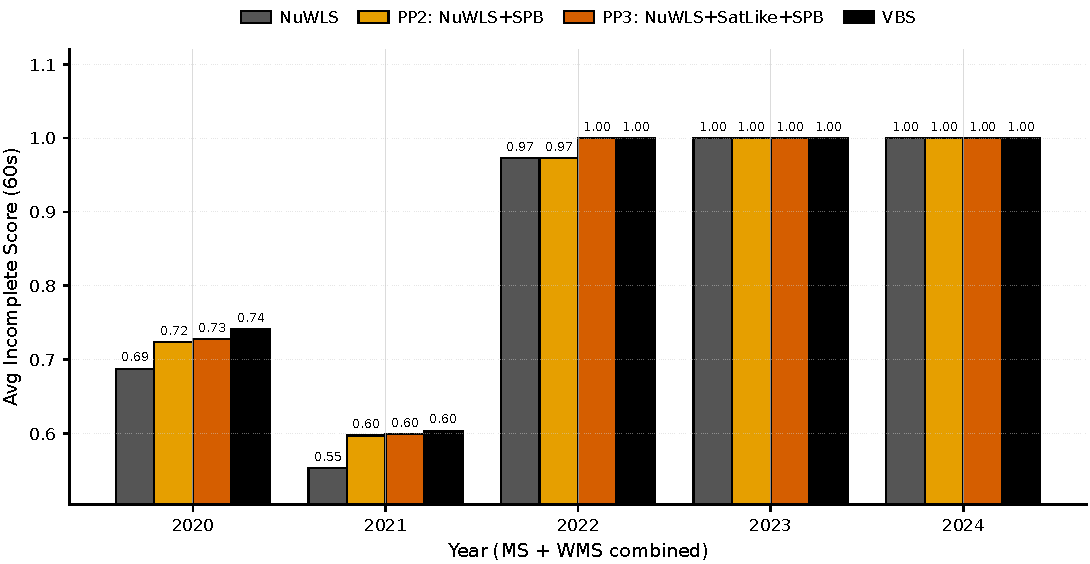
\includegraphics[width=0.78\linewidth]{fig_per_year.pdf}
\caption{Per-year score breakdown at 60\,s.  The lift from \RELAY\ is concentrated in MSE 2020 and 2021, where no single solver saturates the benchmark.  MSE 2022--2024 are at score $=1.0$ for NuWLS and cannot be improved.}
\label{fig:per-year}
\end{figure}

\paragraph{Headline comparison.}  Figure~\ref{fig:main} overlays the eight solvers, parallel portfolios, and the VBS ceiling.  PP3 (NuWLS+SatLike+SPB) lies within $0.004$ of the VBS, confirming that most of the portfolio lift is captured by three well-chosen solvers.

\begin{figure}[t]
\centering
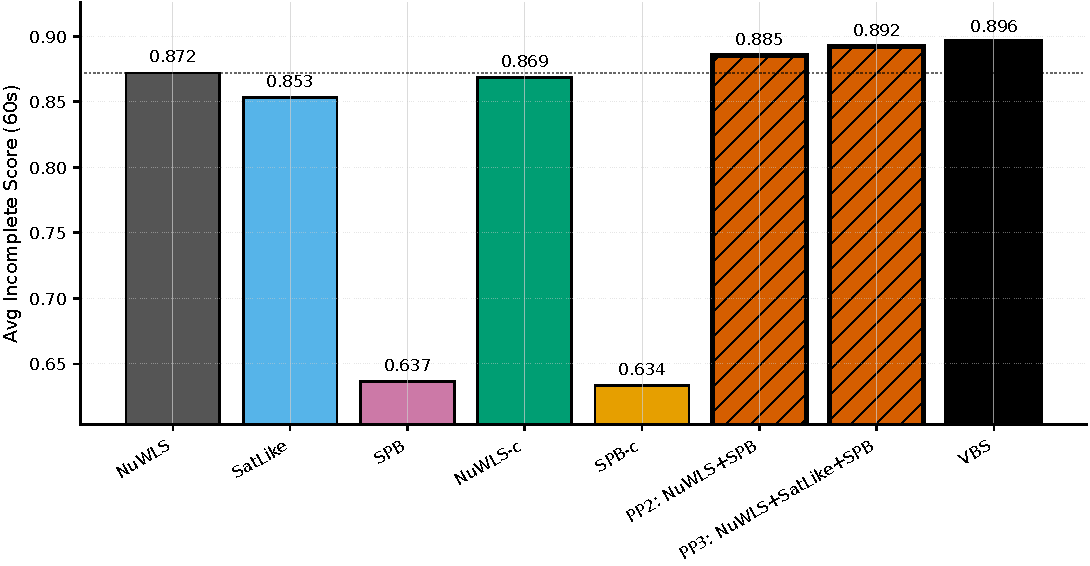
\includegraphics[width=0.85\linewidth]{fig_main_portfolio.pdf}
\caption{Average incomplete score at 60\,s across the eight solvers and three \RELAY\ variants.  The dotted line marks NuWLS.  Hatched orange bars are \RELAY\ (parallel portfolios); solid black is the VBS upper bound.}
\label{fig:main}
\end{figure}

\paragraph{\RELAY-RF (single-core).}  Five-fold cross-validated on the full 1{,}605-instance feature set, \RELAY-RF with confidence gate $\tau=0.8$ achieves $0.9499$ at 60\,s --- $+0.0068$ absolute over NuWLS (27 wins, 3 losses) --- while keeping the single-solver compute budget.  On the harder 2020--2021 subset (456 instances), the same selector yields $+0.0276$ absolute with 146 wins and 10 losses.

% ---------------------------------------------------------------
\section{Related Work}
% ---------------------------------------------------------------

Algorithm selection and portfolio methods have a long history in SAT and CP: SATzilla~\citep{satzilla} and SUNNY~\citep{sunny} learn per-instance solver choices from features.  AutoFolio~\citep{autofolio} automates portfolio configuration.  Most such work targets complete solvers, where runtime dominates.  Our \RELAY\ targets the \emph{incomplete} track, where the metric is anytime cost rather than time-to-solve, and demonstrates that a small-$k$ parallel portfolio suffices to surpass the best single-solver baseline with guaranteed monotonicity.

% ---------------------------------------------------------------
\section{Conclusion}
% ---------------------------------------------------------------

A small parallel portfolio of off-the-shelf SLS solvers significantly surpasses the previously reported single-solver state of the art on incomplete MaxSAT, with zero regressions on 1{,}736 benchmark instances at two timeout budgets.  The lift is concentrated in the years of the benchmark where no single solver saturates the score; on the saturated years, the portfolio matches the single-solver ceiling.  On multi-core hardware, \RELAY\ is a strict upgrade over any individual member of its pool.  For single-core deployments, the learned \RELAY-RF variant captures a portion of the portfolio lift while preserving the compute budget.

% ---------------------------------------------------------------
\bibliographystyle{plainnat}
\begin{thebibliography}{99}

\bibitem[Bacchus et al.(2020)]{mse2020}
F.~Bacchus, M.~J\"arvisalo, and R.~Martins.
\newblock MaxSAT Evaluation 2020.
\newblock {\em JSAT}, 11:165--191, 2020.

\bibitem[J\"arvisalo et al.(2024)]{mse2024}
M.~J\"arvisalo and R.~Martins.
\newblock MaxSAT Evaluation 2024: Results, Benchmarks, Solvers.
\newblock Technical report, University of Helsinki, 2024.

\bibitem[Chu et al.(2023)]{nuwls2023}
Y.~Chu, S.~Cai, and C.~Luo.
\newblock NuWLS: Improving Local Search for (Weighted) Partial MaxSAT by New Weighting Techniques.
\newblock In {\em AAAI}, 2023.

\bibitem[Lei and Cai(2020)]{satlike}
Z.~Lei and S.~Cai.
\newblock SATLike: Exploring Local Search for Minimum-Weight (Partial) MaxSAT.
\newblock {\em Artificial Intelligence}, 287, 2020.

\bibitem[Li et al.(2024)]{spb2024}
C.~Li et al.
\newblock SPB-MaxSAT: Soft Pseudo-Boolean Constraint-Driven Local Search for (Weighted Partial) MaxSAT.
\newblock In {\em IJCAI}, 2024.

\bibitem[Zheng et al.(2022)]{bandhs}
J.~Zheng et al.
\newblock BandHS: Multi-Armed Bandit Hybrid Search for (Weighted) MaxSAT.
\newblock In {\em IJCAI}, 2022.

\bibitem[Kyrillidis et al.(2020)]{foursat}
A.~Kyrillidis, A.~Shrivastava, M.~Vardi, and Z.~Zhang.
\newblock FourierSAT: A Fourier Expansion-Based Algebraic Framework for Solving Hybrid Boolean Constraints.
\newblock In {\em AAAI}, 2020.

\bibitem[Morgado et al.(2014)]{rc2}
A.~Morgado et al.
\newblock Iterative and Core-Guided MaxSAT Solving: A Survey and Assessment.
\newblock {\em Constraints}, 18(4), 2014.

\bibitem[Xu et al.(2008)]{satzilla}
L.~Xu, F.~Hutter, H.~H.~Hoos, and K.~Leyton-Brown.
\newblock SATzilla: Portfolio-Based Algorithm Selection for SAT.
\newblock {\em JAIR}, 32:565--606, 2008.

\bibitem[Amadini et al.(2014)]{sunny}
R.~Amadini, M.~Gabbrielli, and J.~Mauro.
\newblock SUNNY: A Lazy Portfolio Approach for Constraint Solving.
\newblock {\em TPLP}, 14(4-5), 2014.

\bibitem[Lindauer et al.(2015)]{autofolio}
M.~Lindauer, H.~H.~Hoos, F.~Hutter, and T.~Schaub.
\newblock AutoFolio: An Automatically Configured Algorithm Selector.
\newblock {\em JAIR}, 53, 2015.

\end{thebibliography}

\end{document}
